%\documentclass[fleqn, letterpaper]{amsart}
\documentclass[fleqn, letterpaper]{tufte-handout}
\usepackage{times}
\usepackage{amsmath}
\usepackage{graphicx}
\usepackage{booktabs}
\usepackage{multirow}
\usepackage{listings}
\usepackage{epstopdf}
%\usepackage[left=1in]{geometry}

\newcommand{\R}{\mathcal{R}}
\newcommand{\E}{\text{E}}
\newcommand{\p}{p_{XY}}
\renewcommand{\arraystretch}{1.5}

\title{Problem Set 3 --- ENCE689E Spring 2014}
\author{David Prentiss}

\begin{document}
\maketitle

\section{1. Monte Carlo Methods}
\subsection{(a)}
\begin{figure}
    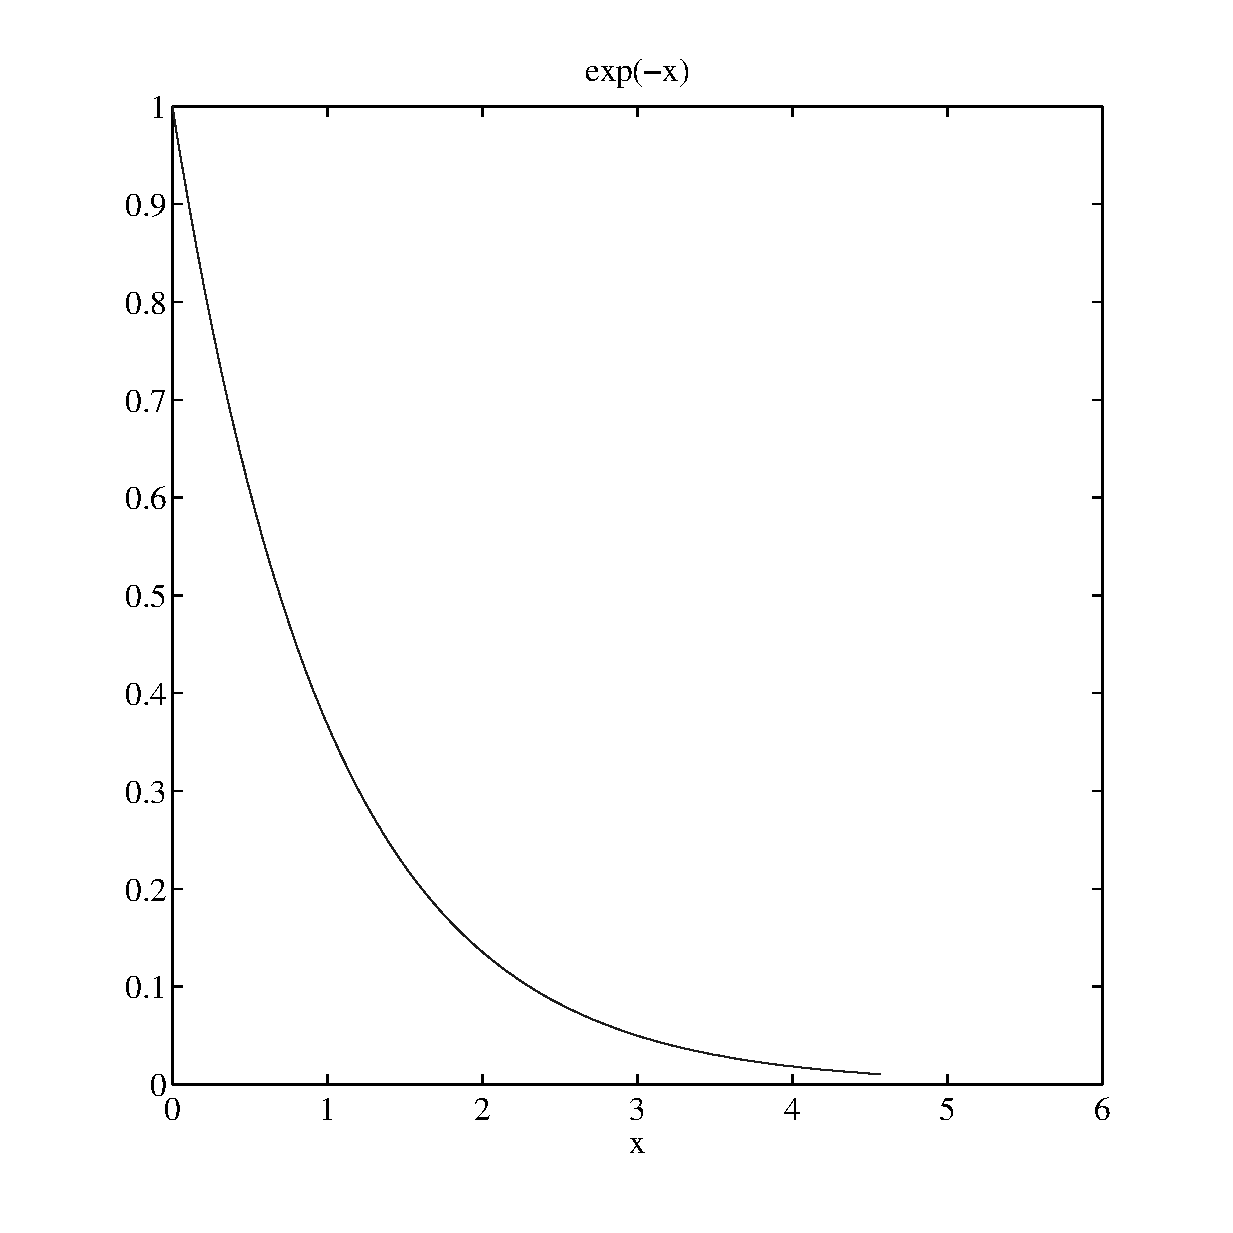
\includegraphics[width=\textwidth]{problem1a}
    \caption{Plot of $p_X(x)=e^{-x}$}
    \label{exprnd}
\end{figure}

\subsection{(b)}
    \[
    P_X(x) = \int_{-\infty}^x p_X dx
     = 0 + \int_0^x p_X dx = 1 - e^{-x}
    \]

\[
P^{-1}_X = -\ln(1-P_X(x))
\]
\subsection{(c), (d)}
See Figures \ref{rand} and \ref{exprnd} and Listing \ref{lst1}. \\
\begin{figure}
    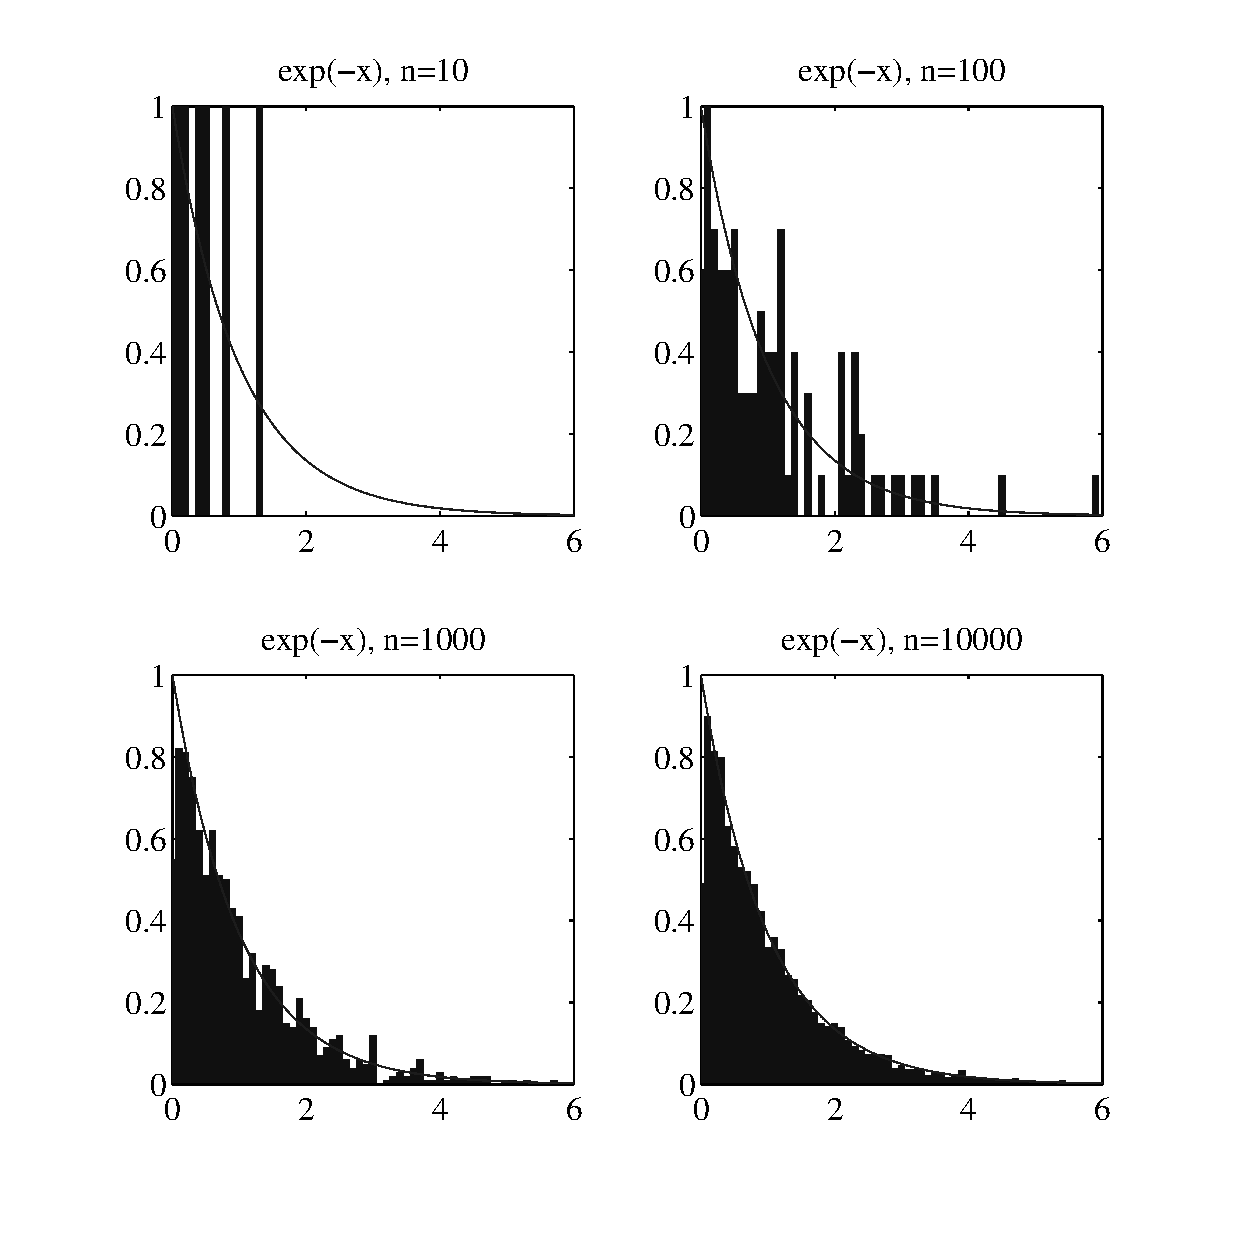
\includegraphics[width=\textwidth]{problem1}
    \caption{Ensebles generated with the inverse cumulative distribution function.
    For the ensemble with $n=1000$ the sample mean and variance are $0.9882$ and $0.9590$ respectively.}
    \label{rand}
\end{figure}
\begin{figure}
    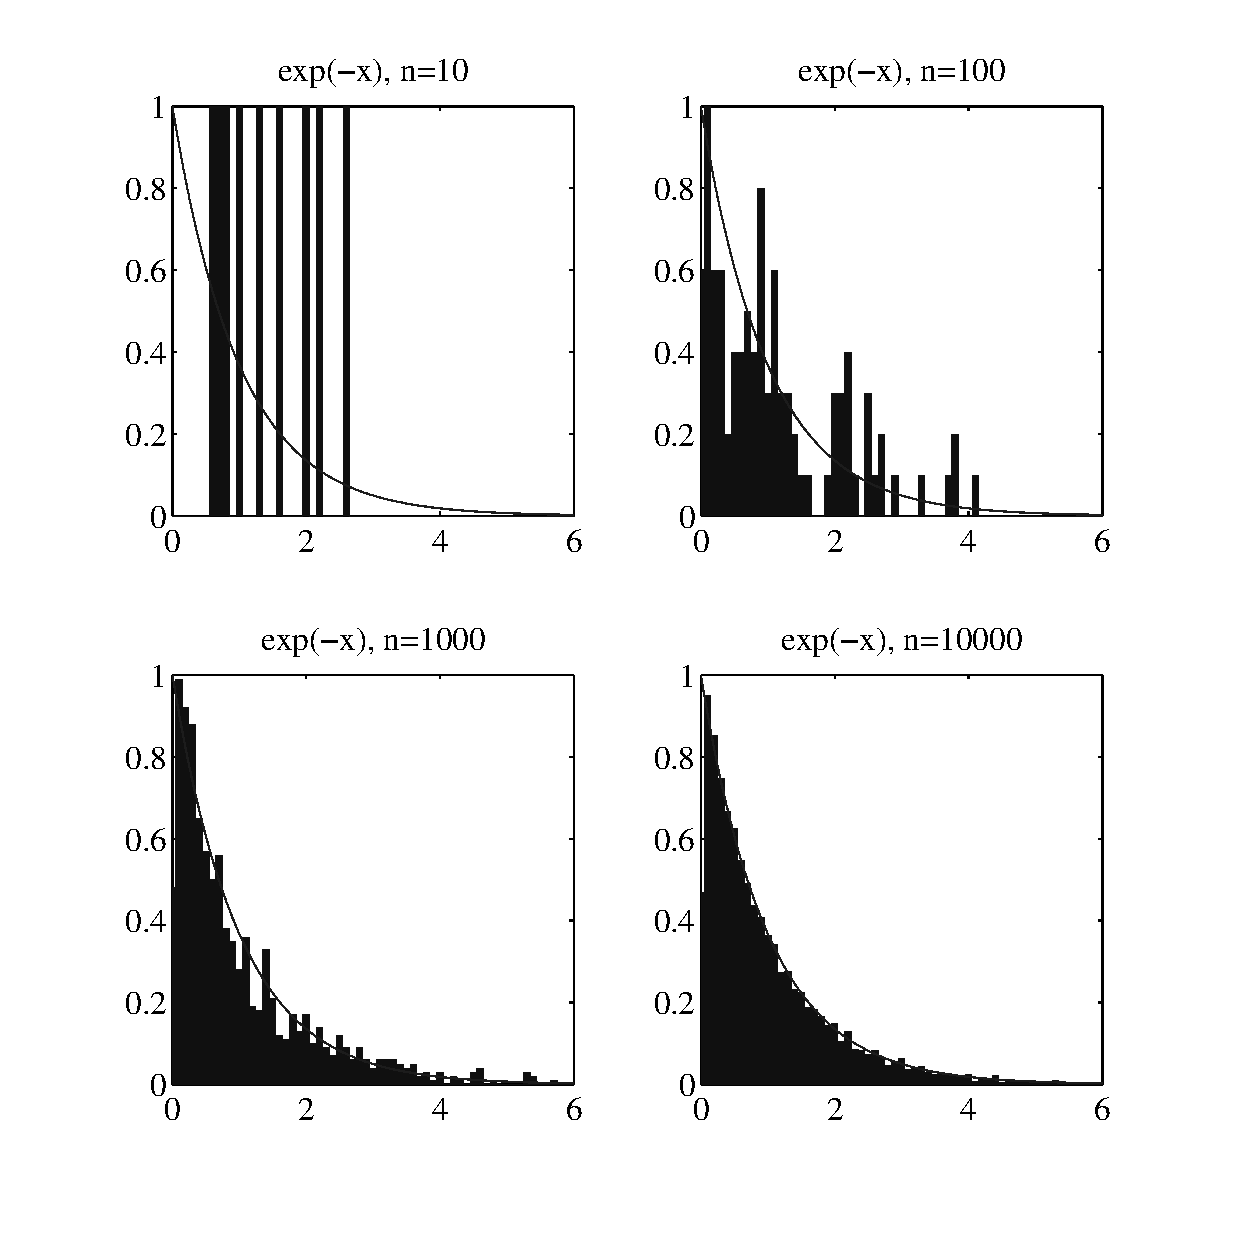
\includegraphics[width=\textwidth]{problem1e}
    \caption{Ensebles generated with the MATLAB {\ttfamily exprnd} function.
    For the ensemble with $n=1000$ the sample mean and variance are $0.9904$ and $1.0043$ respectively.}
    \label{exprnd}
\end{figure}
\small
\begin{minipage}{\linewidth}
\lstinputlisting[language=Matlab, caption={Monte Carlo estimation of $e^{-x}$ in MATLAB},
 basicstyle=\ttfamily, label=lst1]{ps3problem1.m}
\end{minipage}
\subsection{(e)}

\section{2. Monte Carlo Methods}
\subsection{(a)}
\subsection{(b)}
\subsection{(c)}
\begin{figure}

    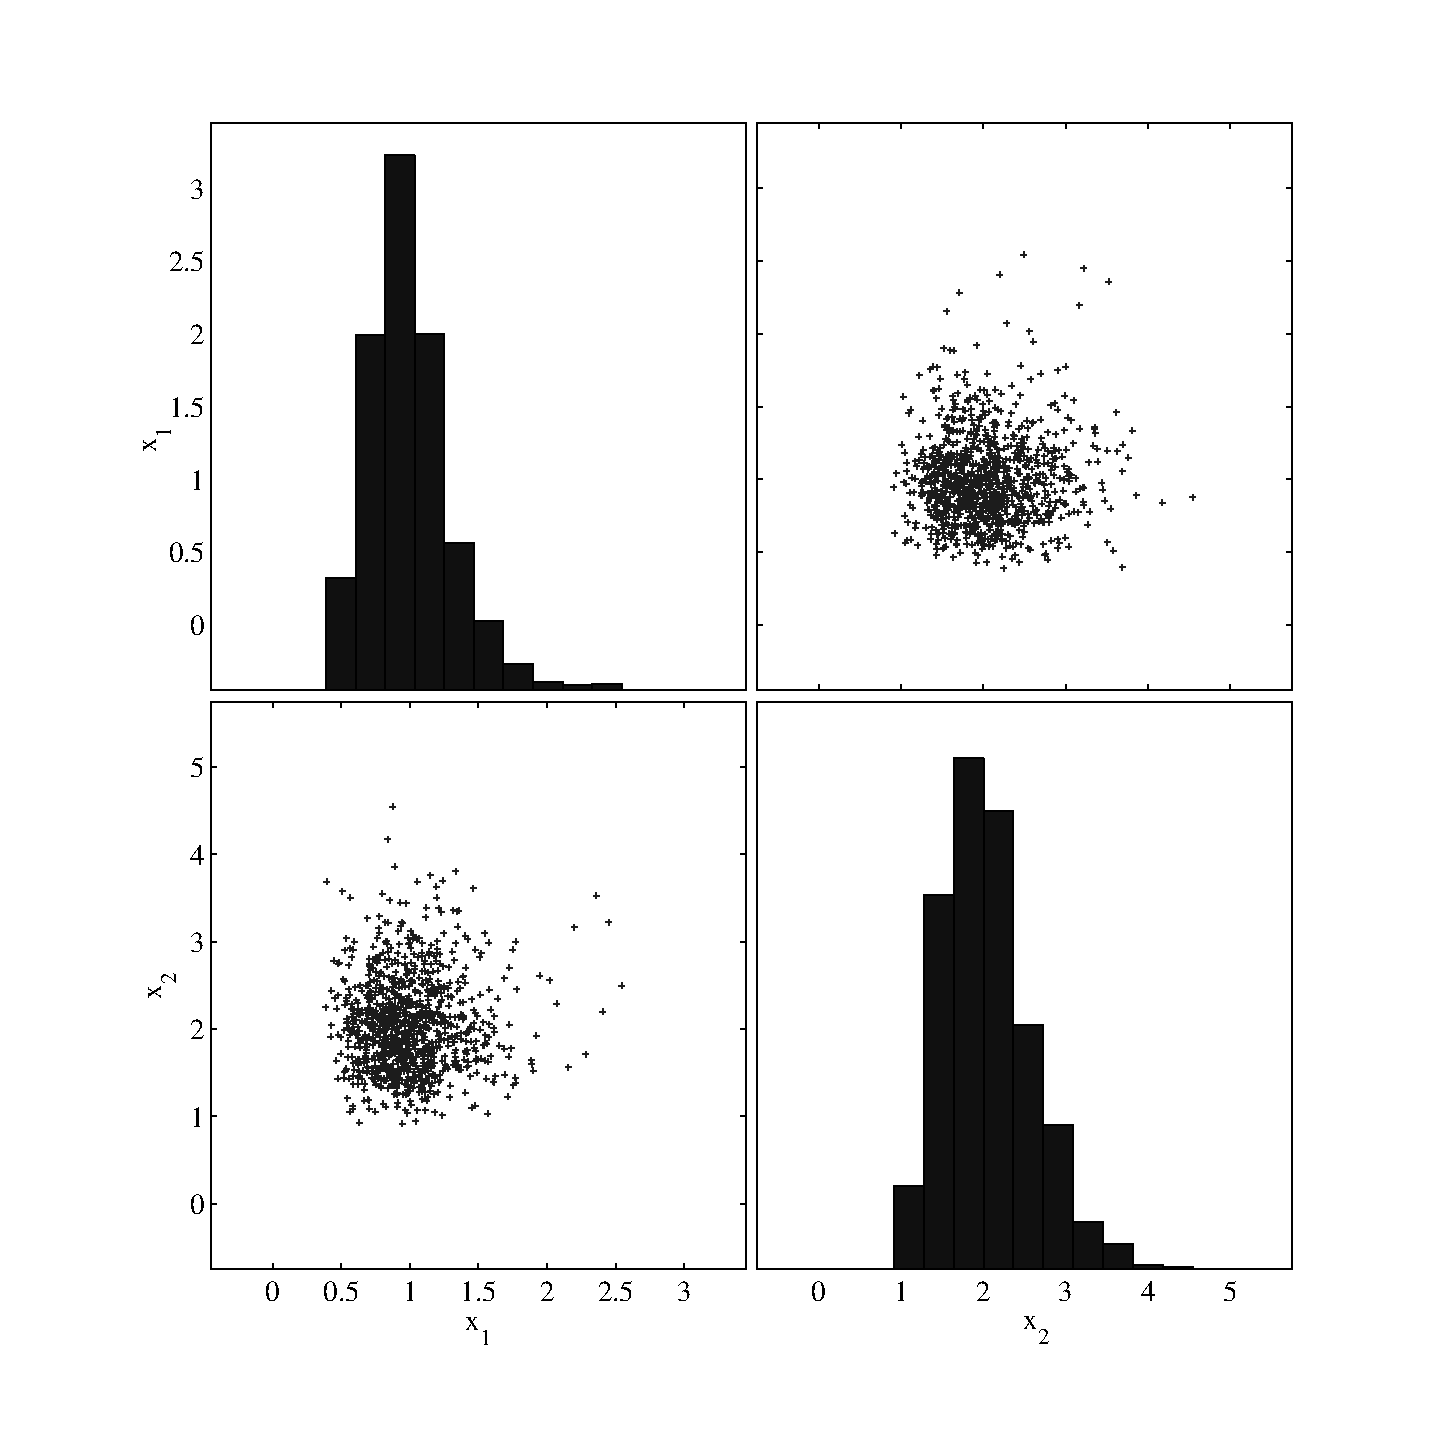
\includegraphics[width=\textwidth]{problem2}
    \caption{Ensebles generated with the matlab {\ttfamily exprnd} function}
    \label{norm}
\end{figure}
\subsection{(d)}
\begin{minipage}{\linewidth}
\lstinputlisting[language=Matlab, basicstyle=\ttfamily]{ps3problem2.m}
\end{minipage}
\subsection{(e)}
\begin{figure}
    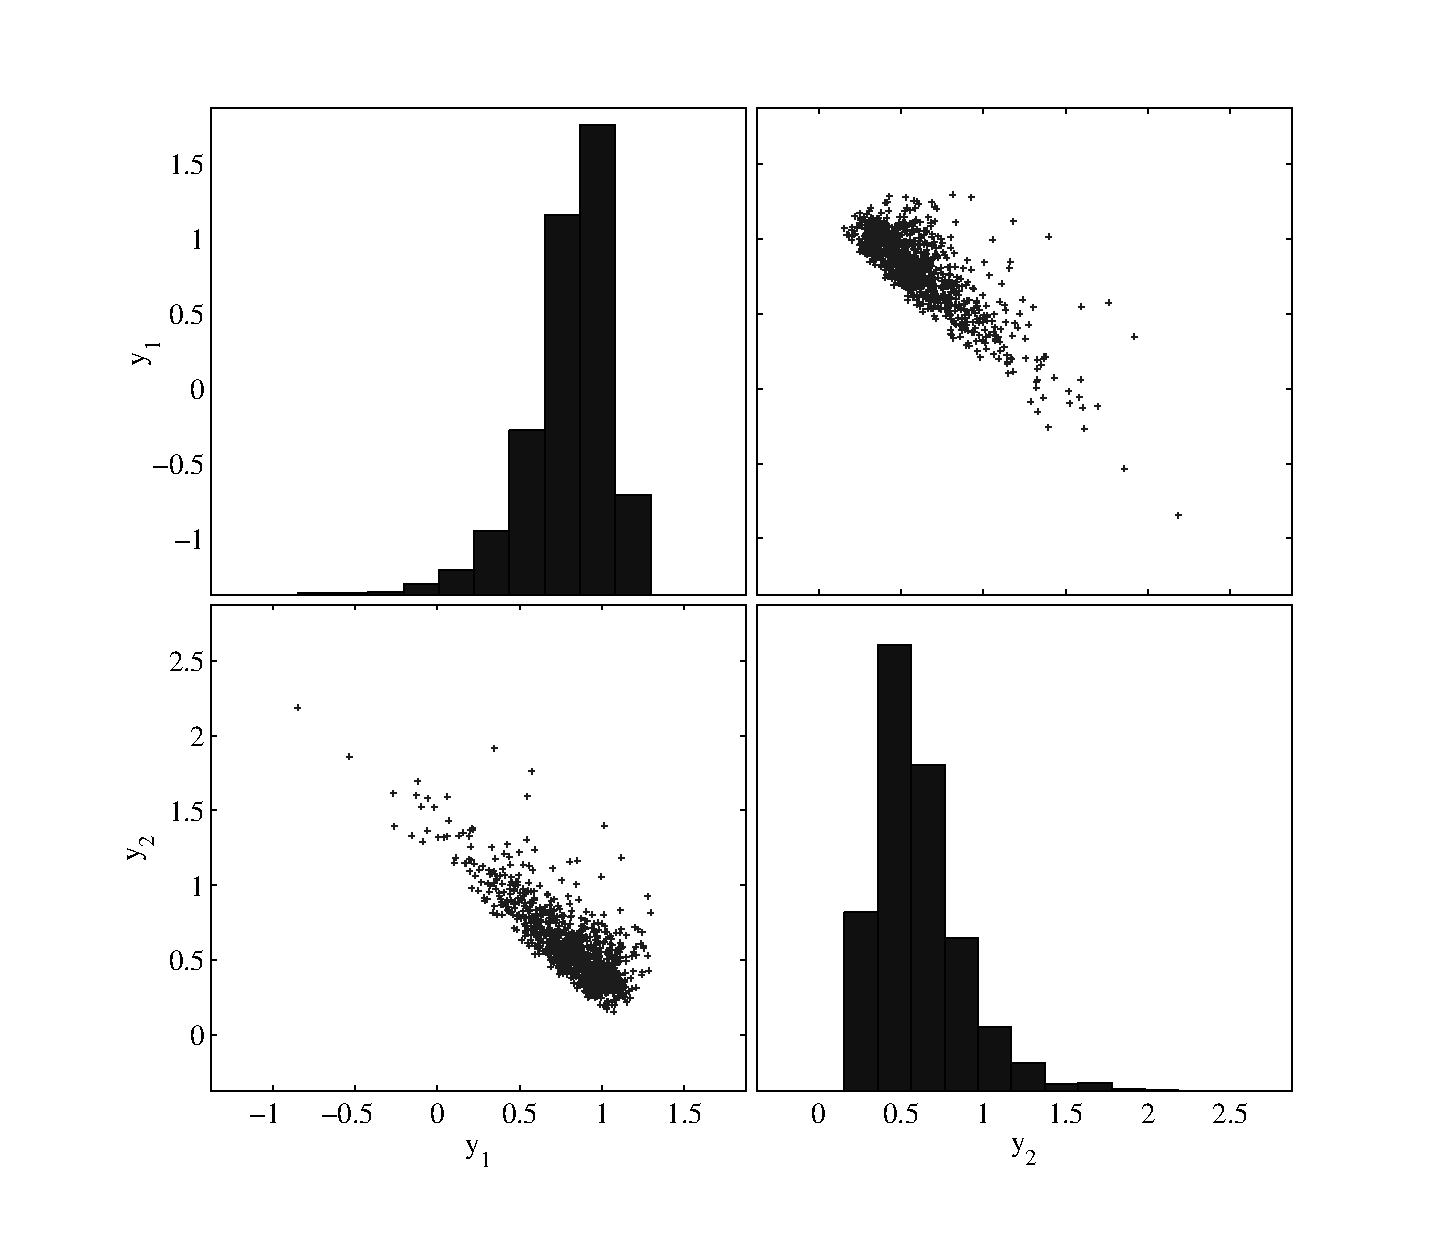
\includegraphics[width=\textwidth]{problem2e}
    \caption{Ensebles generated with the MATLAB {\ttfamily exprnd} function}
    \label{lognorm}
\end{figure}

\end{document}